\documentclass[a4paper]{article}
\usepackage[T1]{fontenc}
\usepackage[utf8x]{inputenc}
\usepackage[english,russian]{babel}
\usepackage{multicol}
\usepackage{fancyhdr}
\usepackage[warn]{mathtext}
\usepackage{graphicx}
\usepackage{microtype}
\usepackage{wrapfig}
\usepackage{amsmath}
\usepackage{floatflt}
\usepackage{geometry} \geometry{verbose,a4paper,tmargin=2cm,bmargin=2cm,lmargin=1.5cm,rmargin=1.5cm}
\usepackage{float}
\usepackage{amssymb}
\usepackage{caption}
\usepackage{epsfig}
\usepackage{newunicodechar}

\begin{document}
\newcommand{\apple}{\char"F8FF}

\begin{titlepage}
	\centering
	\vspace{5cm}
    {\scshape\LARGE Московский физико-технический институт\par}
    
\begin{figure}[H]
\begin{center}

\includegraphics[scale = 0.4]{mipt_rus_text.png}
\label{default}
\end{center}
\end{figure}

	\vspace{3cm}
	{\scshape\Large Лабораторная работа по вакуумной электронике \par}
	\vspace{1cm}
    {\huge\bfseries  Автоэлектронная эмиссия \par}
	\vspace{1cm}
	\vfill
\begin{flushright}
	{\large выполнил студент Б04-852 группы ФЭФМ}\par
	\vspace{0.3cm}
	{\LARGE Яромир Водзяновский}
\end{flushright}
	
	\vfill
Долгопрудный, 2020
% Bottom of the page
\end{titlepage}

\pagestyle{fancy} 
\fancyhead[R]{Автоэлектронная эмиссия}
\fancyhead[L]{Вакуумная электроника}
\fancyhead[C]{}
\fancyfoot[C]{ \noindent\rule{\textwidth}{0.4pt} \thepage }

\newpage


\section{Цель работы}

\begin{itemize}
	\item Изучить целти и особенности автоэлектронной эмиссии и ее приминения
	\item Ознакомится с техникой автоэлектронной микроскопии и областями ееприминения, а также 
	с методикой получения острий для автоэлектронных микроскопов
	\item Исследовать автоэмиссионные свойства катода из углеродных волокон, а также механихмы
	нестабилности автоэмиссионного тока в нем.
\end{itemize}

\section{Теория}

При наличии электростатического поля над поверхностью металла наблюдается внешнаяя автоэлектронная 
эмиссия или просто \textbf{автоэмиссия}.

\textbf{Автоэлектронной эмиссией} называется явление испуская электронов в вакуум с поверхности
твердого тела и другой среды под действием оцень сильгного электрического поля напряженностью 
$E = 10^7 - 10^8$(В/см).

Для того чтобы создать такие сильные жлектрические поля, к обычным макроскопическим электродам 
необходимо приложить напряжение в десятки миллион эВ. Практически автоэлектронную эмиссию можно 
возбудить при гораздо меньших напряжениях, если придать катоду форму тонкого острия с радиусом
вершины в десятые или сотые доли микрона. Сейчас реализованы условия, когда при микроскопических
расстояниях катод-анод, равных единицам или долям микрона, и очень малых радиусах кривизны катода 
$z = 20 - 50 A (1 A = 10^{-8}cm)$.

Автоэлектронная эмиссия не требует возбуждения электронов. Суть явления состоит в туннелировании
электронов сквозь потенциальных барьер на поверхности тела. Такое туннелирование становиться возможным
за счет искривления потенциального барьера при приближении электрон может существовать с той же 
полной энергией которой он обладает, находясь в теле. Таким образом, автоэлектронная эмиссия обусловлена
волновыми свойствами электонов. Впервые такое объяснение автоэмиссии было предложено в 1928 году 
Фаулером и Нордгеймом. Ими впервые была получена формула, описывающая взаимосвязь плотности 
автоэлектронного тока $j$ с напряженностью $E$:
$$j = \frac{e^3}{4 \pi^2 \hbar} \cdot \frac{E_f^{1/2}}{W_a \phi^{1/2}} \cdot E^2 \cdot \exp{\left( - \frac{4 \sqrt{2m}}{3e\hbar} \cdot \frac{\phi^{3/2}}{E} \right)}$$

где $W_a - E_f$ - работа выхода, $E_f$ - энергия Ферми, $W_a$ - уровень вакуума. Вся энергии отсчитываются
от дна зоны проводимости.
Эта формула получена для полубесконечного металла с плоской поверхностью, подчиняющегося модели 
Зоммерфельда и находящегося при температуре $T = 0 (K)$. 

\section{Оборудование}

В работе используется следующая установка:

\begin{figure}[h]
	\begin{center}
	\begin{minipage}[h]{0.45\linewidth}
	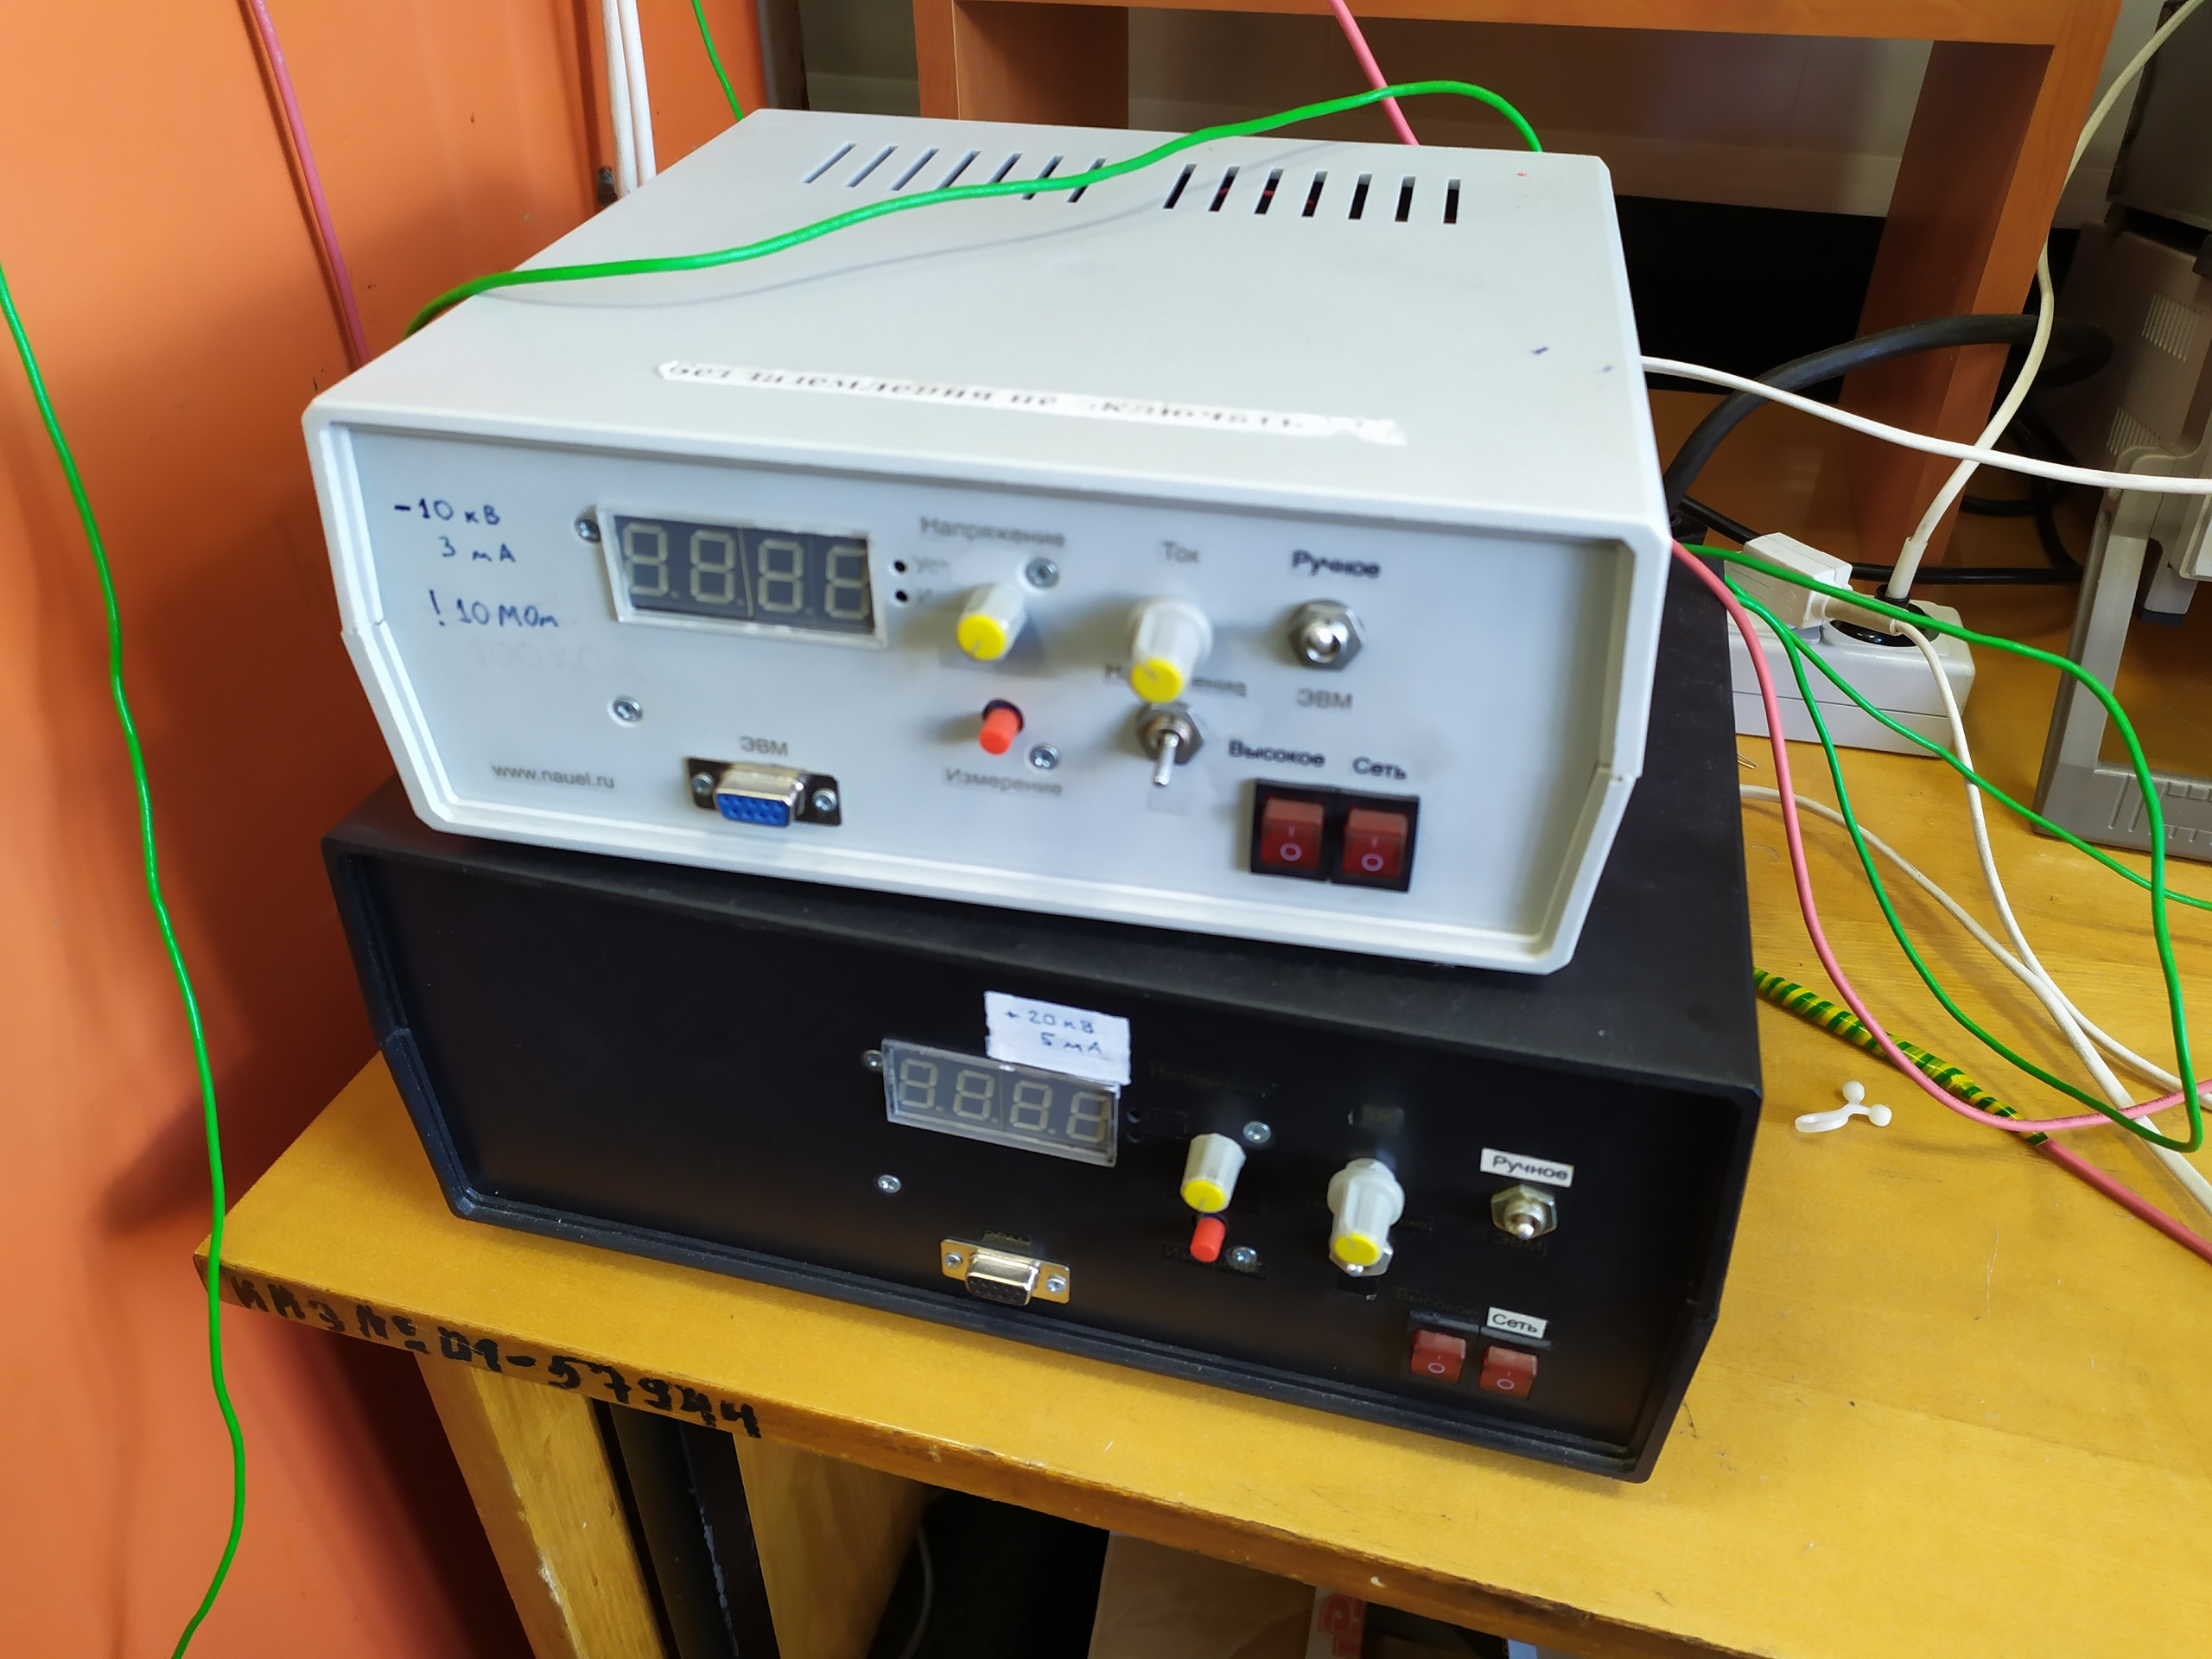
\includegraphics[width=1\linewidth]{p2.jpg}
	\caption{Измеритель тока и вольтметр} 
	\label{p2}
	\end{minipage}
	\hfill 
	\begin{minipage}[h]{0.45\linewidth}
	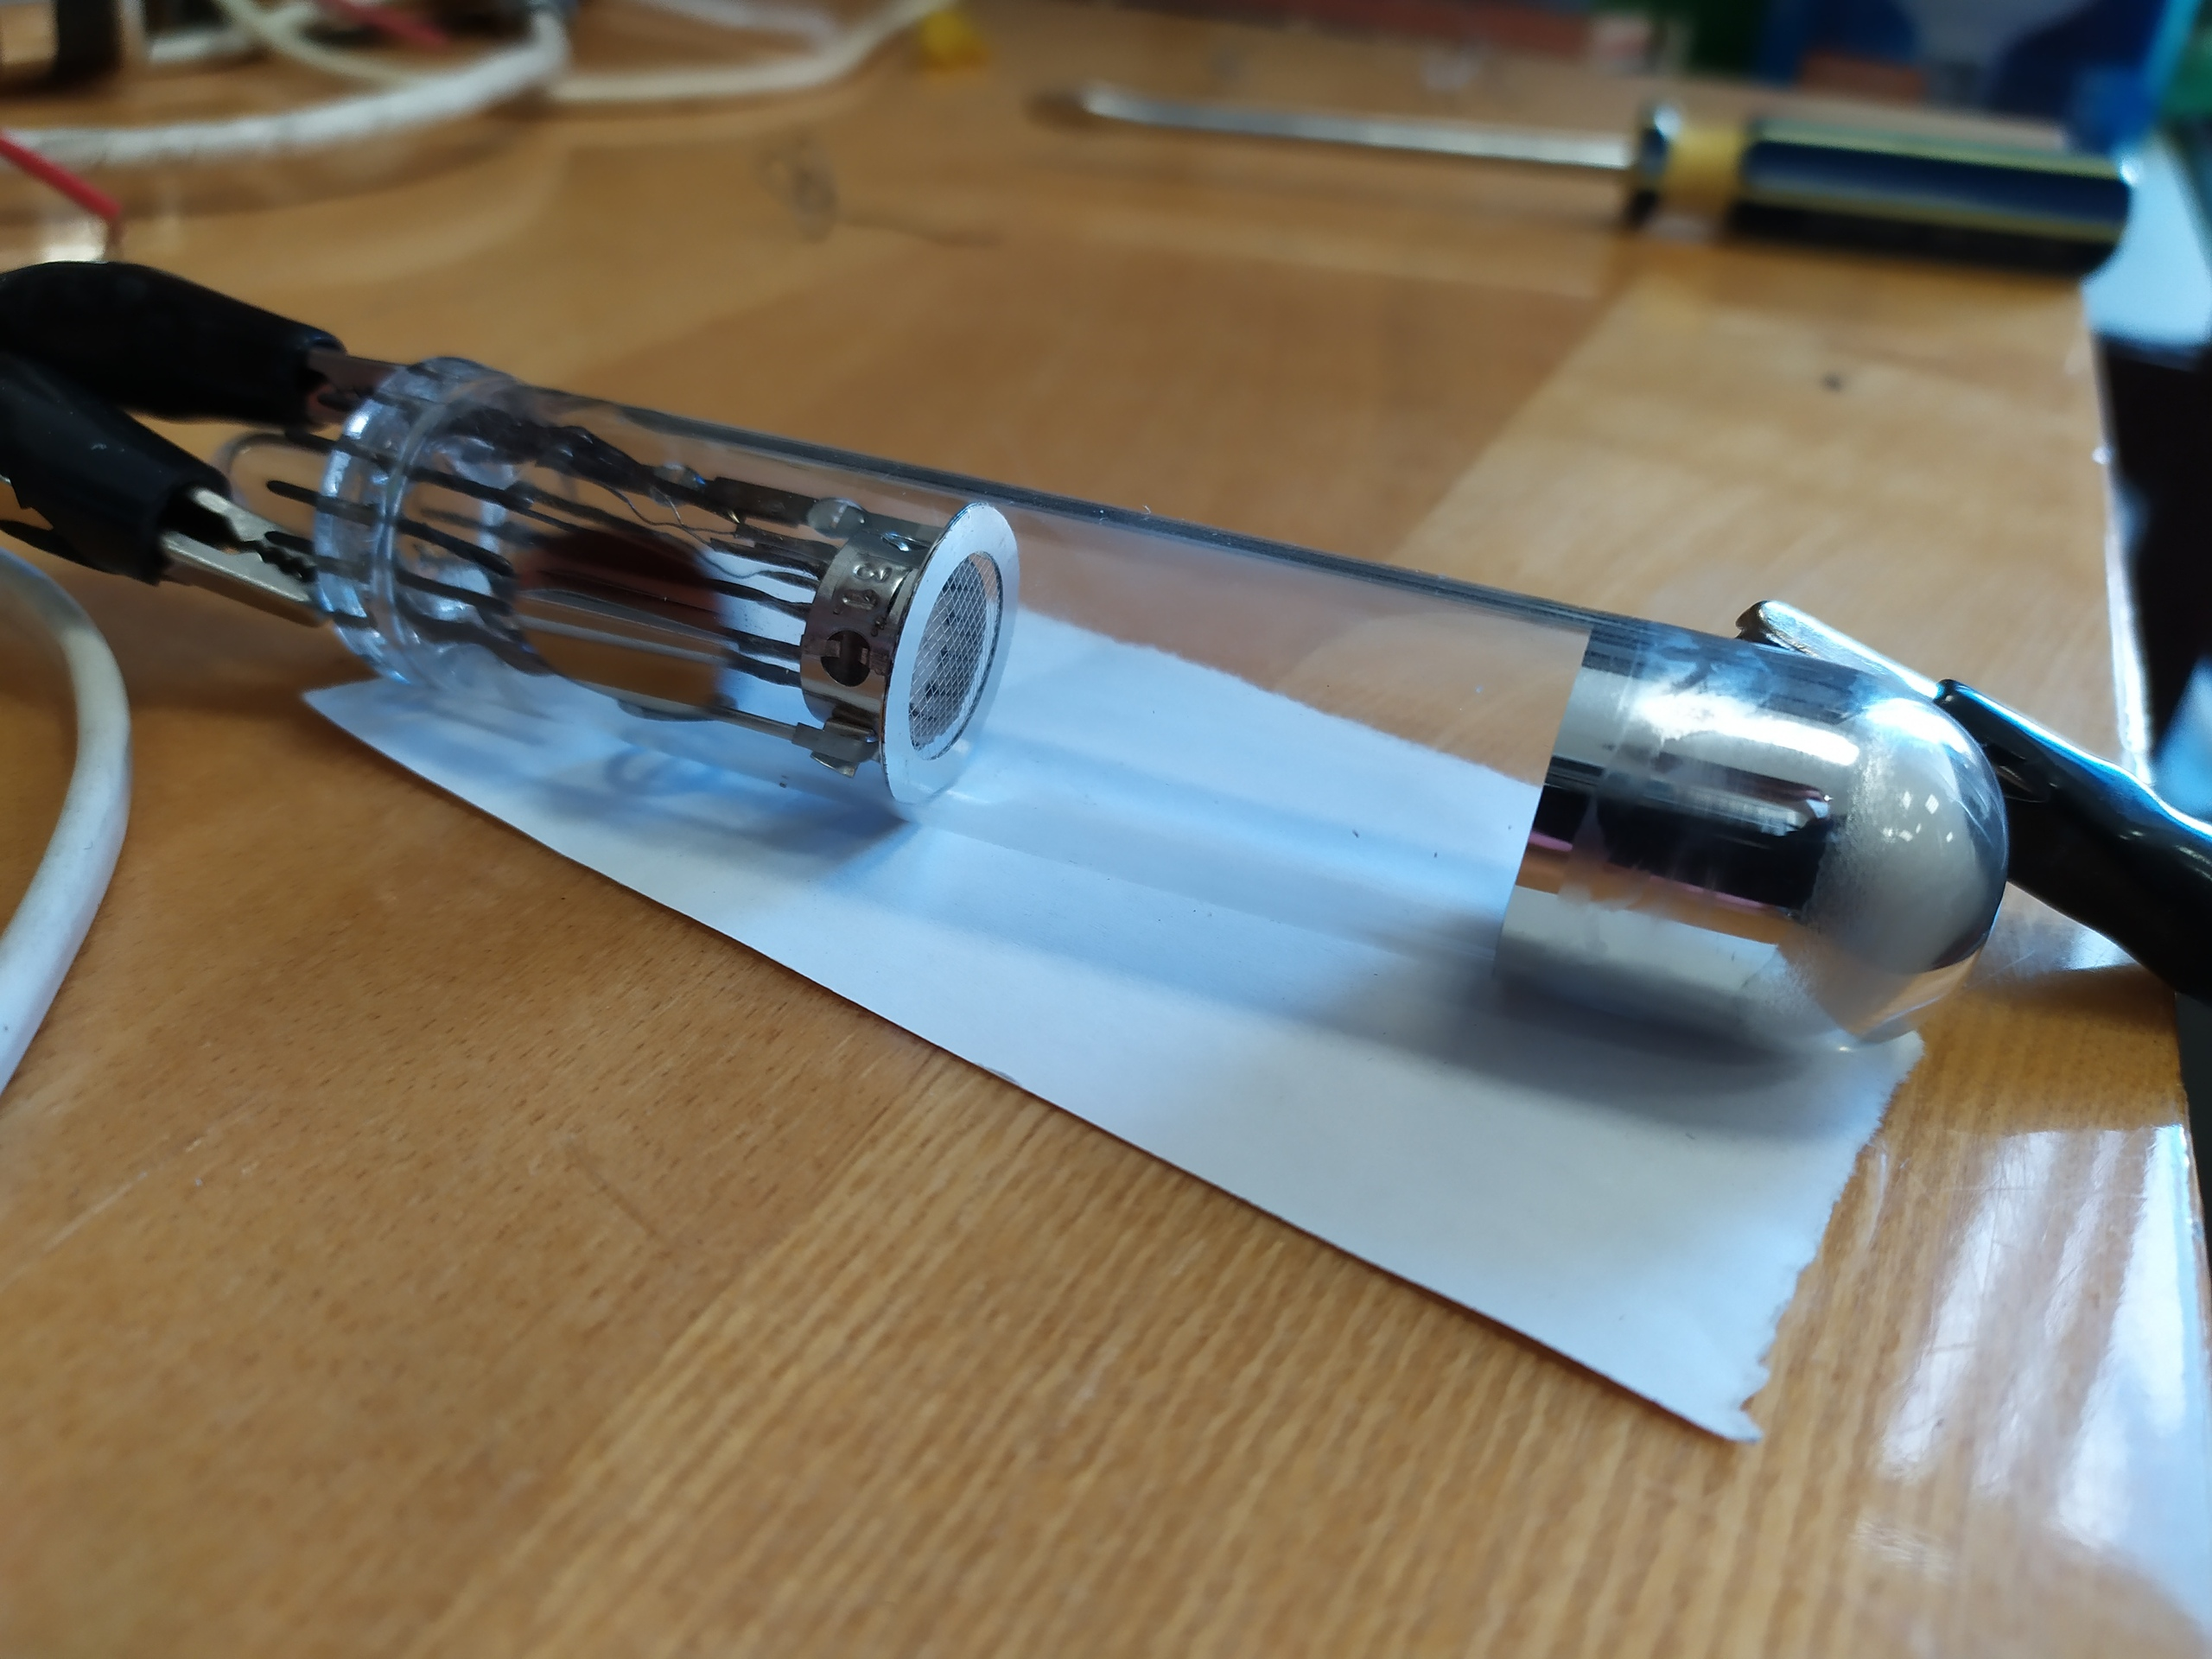
\includegraphics[width=1\linewidth]{p1.jpg}
	\caption{Диод}
	\label{p2}
	\end{minipage}
	\end{center}
\end{figure}

\begin{figure}[H]
	\begin{center}
	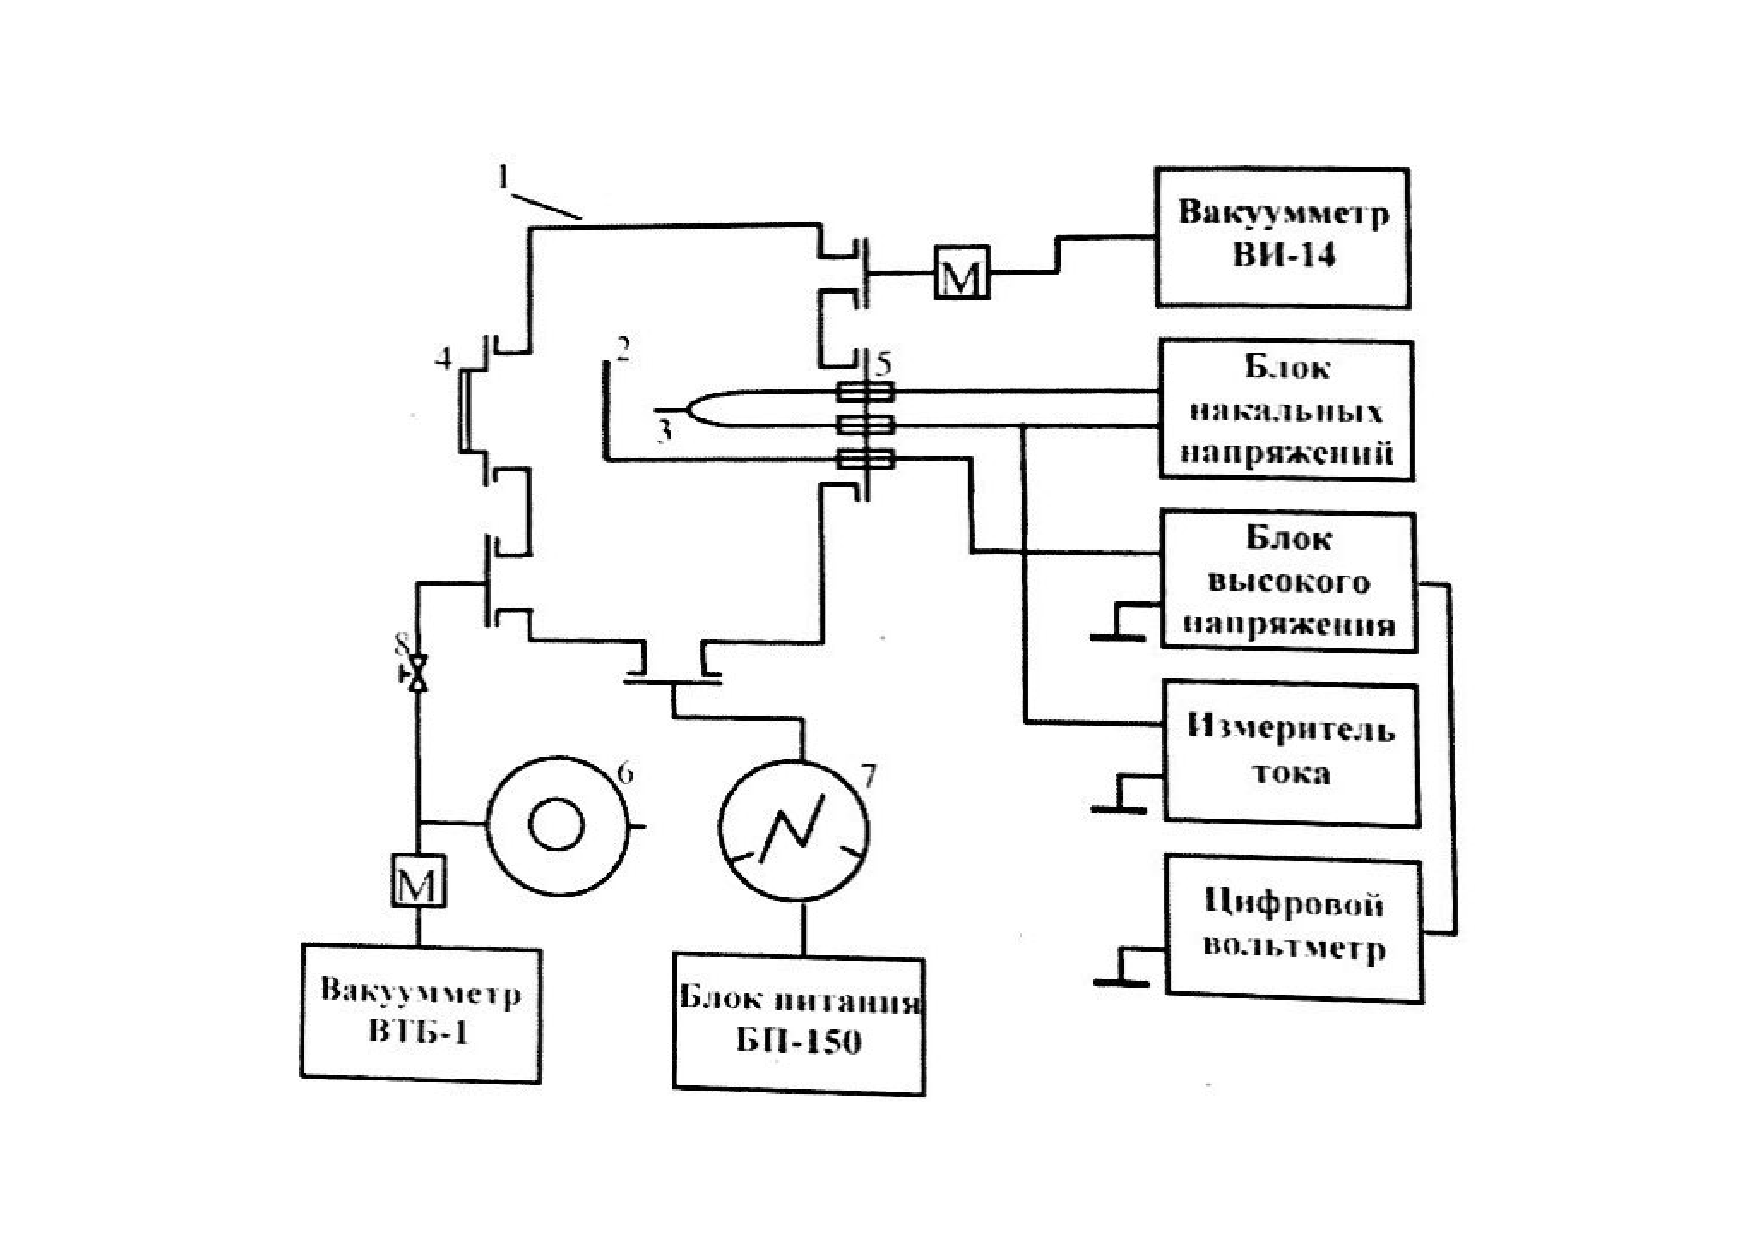
\includegraphics[scale = 0.35]{p3.pdf}
	\caption{Блок-схема установки}
	\label{default}
	\end{center}
\end{figure}

1 - вакуумная камера, 2 - анод, 3 - исследуемы образец, 4 - смотровое окно, 5 - 
фланец с высоковольтными выводами, 6 - цеолитовый насос, 7 - магниторазрядный насос.

\section{Ход работы}

\begin{enumerate}
	\item Снимем зависимость силы тока от напряжения при возрастании напряжения 
	начиная с точки, где навчинаяется свечение образца
	\begin{table}[H]
        \centering
        \caption{}
        \label{t1}
        \begin{tabular}{|c||c|c|c|c|c|c|c|c|c|c|c|c|c|c|}
            \hline
			U, кВ&2.20&2.25&2.30&2.35&2.40&2.45&2.50&2.55&2.60&2.65&2.70&2.75&2.80&2.85 \\ \hline
			I, мА&0&0.01&0.01&0.01&0.02&0.02&0.02&0.03&0.03&0.04&0.06&0.08&0.13&0.02 \\ \hline
        \end{tabular}
    \end{table}

	В момент перехода от 2.8 кВ к 2.85 кВ ток резко упал до 0.02 мА. Скачек тока 
	сопровождался щелчком, с этого момент ана аноде наблюдалось яркое свечение.

	\item Построим график зависимости I(U) и сделаем фит экспонентой:

	\begin{figure}[H]
		\begin{center}
		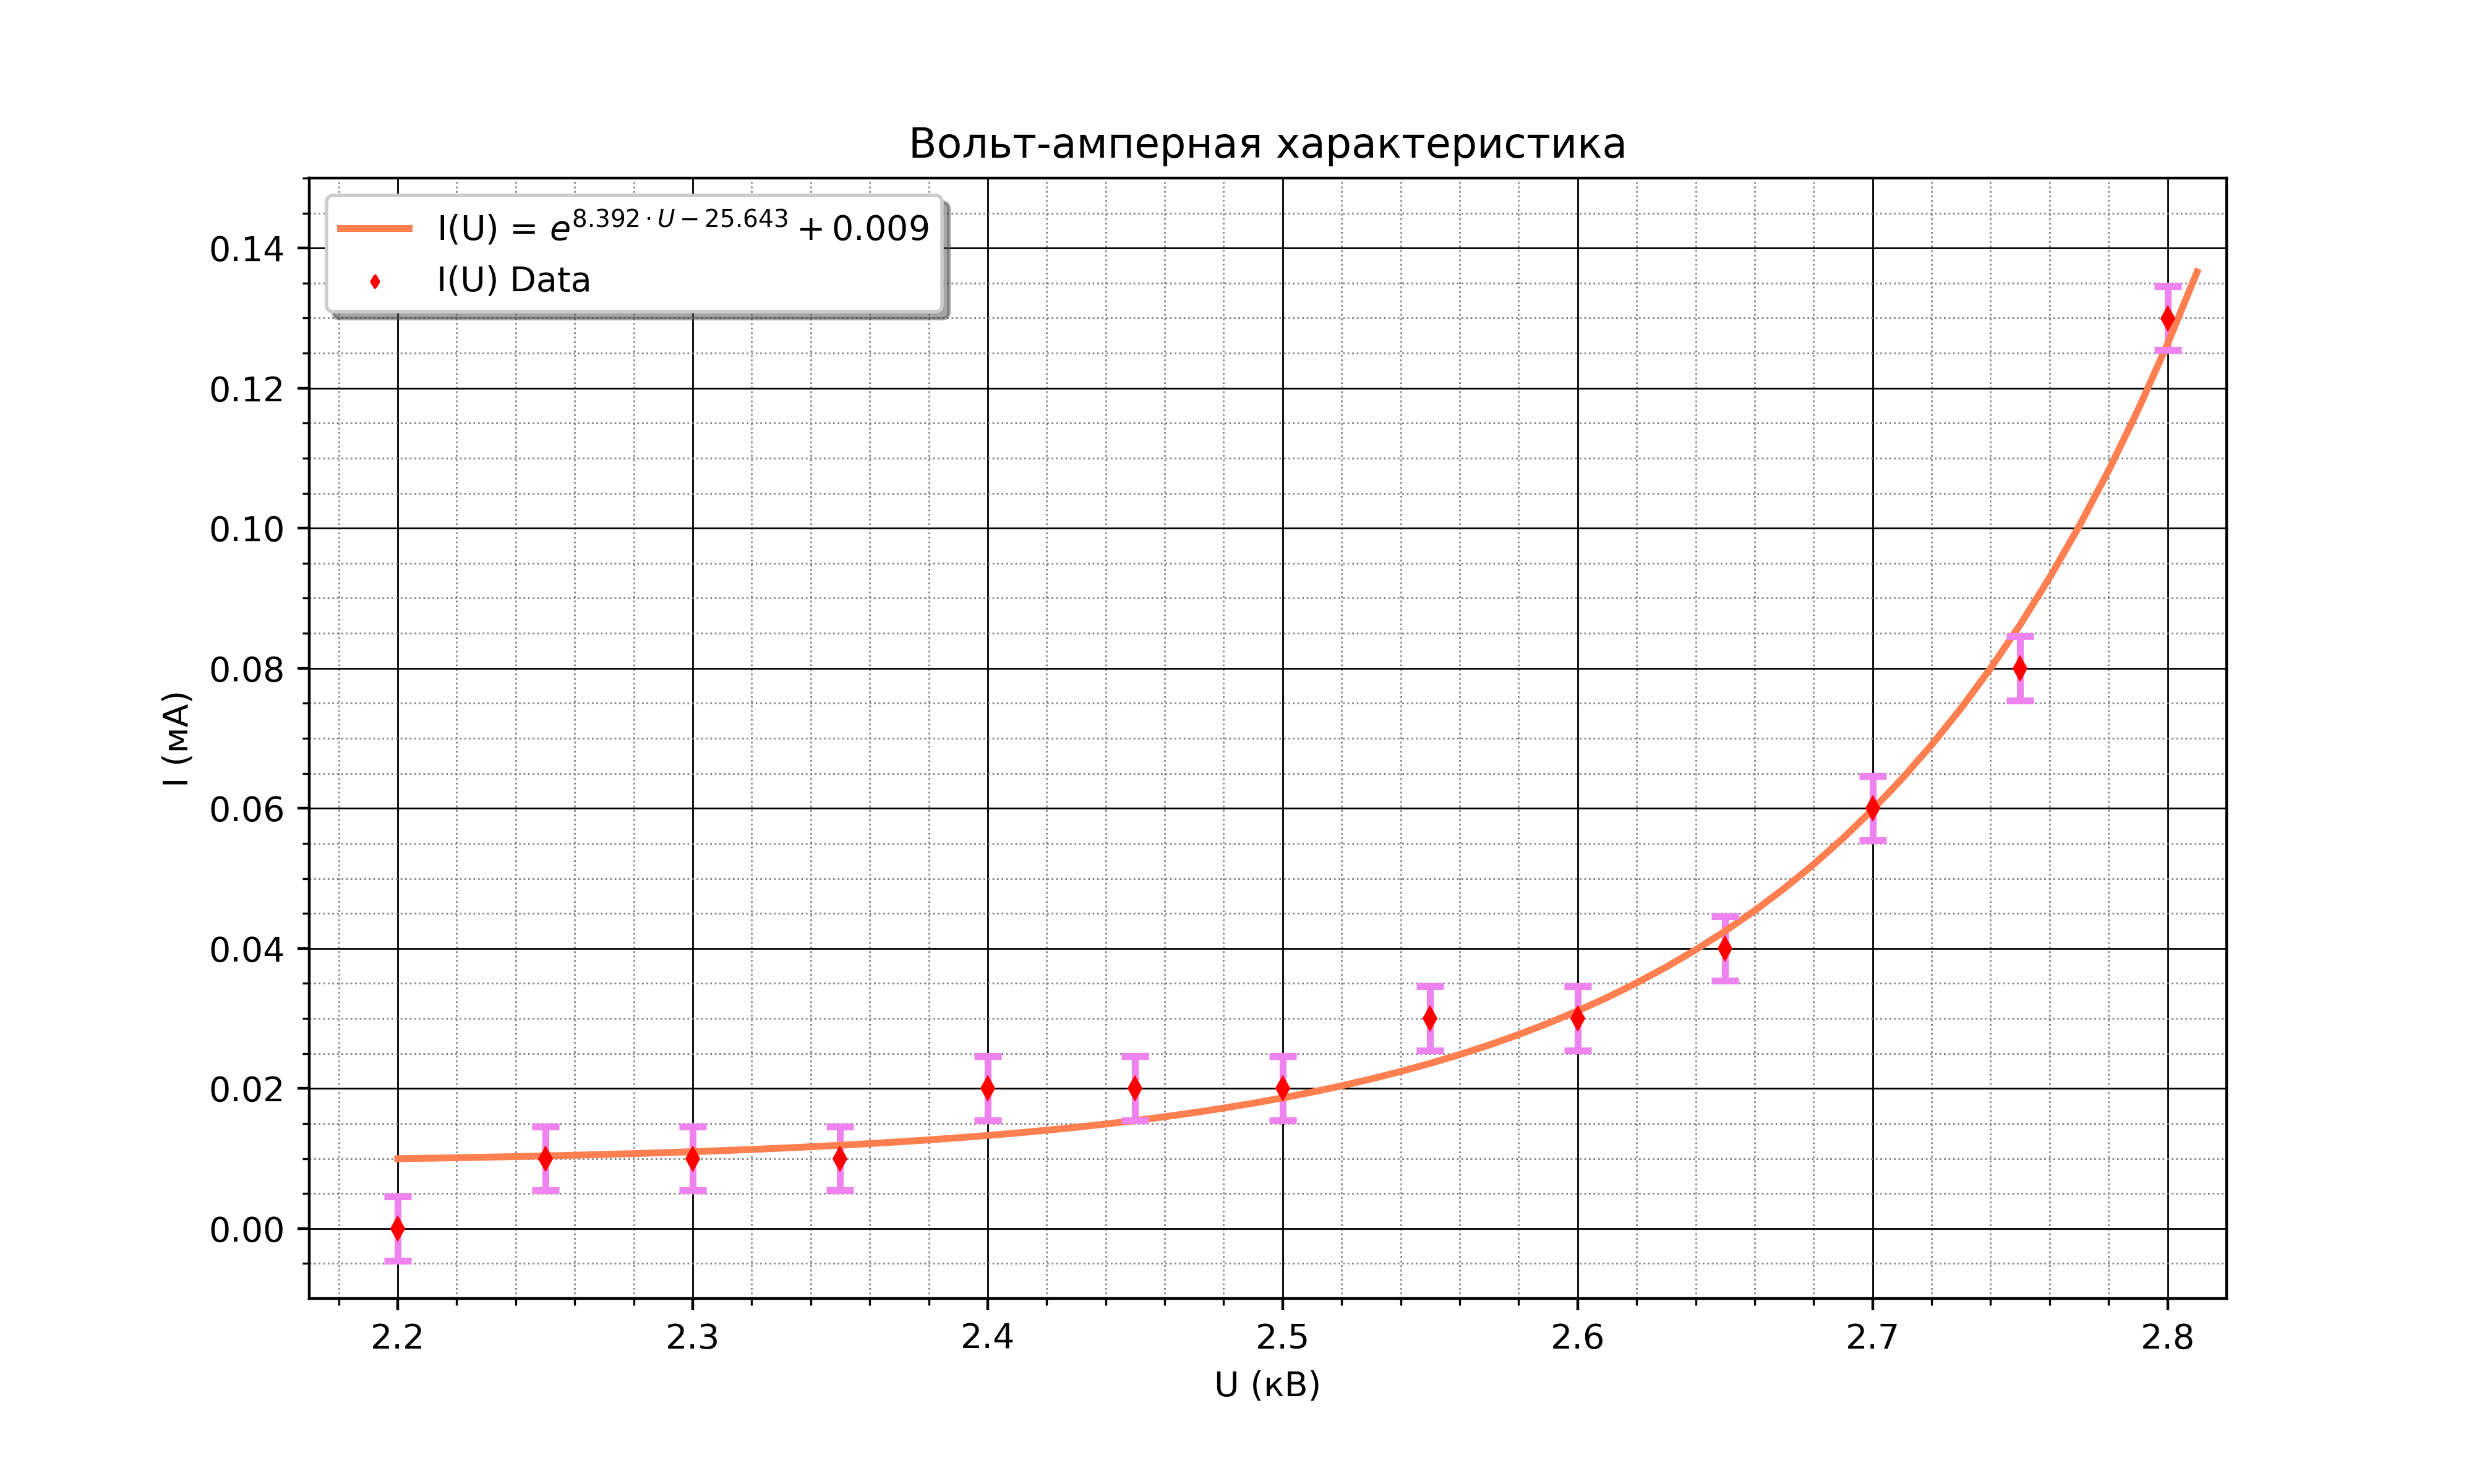
\includegraphics[scale = 0.5]{I(U).png}
		\caption{ВАХ фит exp}
		\label{default}
		\end{center}
	\end{figure}

	Погрешность по вертикали $\sim 0.0046$ мА.
	
	\item Пересчитаем координаты в координаты Фаулера-Нордгейма $\ln{\left( \frac{I}{U^2} \right)}$
	от $\frac{1}{U}$

	\begin{figure}[H]
		\begin{center}
		\includegraphics[scale = 0.6]{LN.png}
		\caption{ВАХ в координатах Фаулера-Нордгейма}
		\label{default}
		\end{center}
	\end{figure}

	Ошибка по вертикали $\sim 0.215$

\end{enumerate}

\section{Ответы на контрольные вопросы}

\begin{enumerate}
	\item \textbf{Расскажите о травлении углеродных трубок}
	\begin{itemize}
		\item В ходе опытов установилось, что у автоэмиссионного катода происходит отклонение периферийных волокон под действием 
		электростатических сил. В результате механического колебания вохможен отрыв отдельных волокон из пучка. 
		Оторванные волокна могут закоротить межэлектронный промежуток катод-модулятор. Во избежание этого необходимо 
		придать катоду форму, которая обеспечит одинаковое электроическое поле у волокон в пучке. 

		\item Выбран метод травления катодного пучка углеродных волокон коронным разряжом в воздухе, т.к. коронный разряд
		близок по своей сути к автоэмиссии. Действие коронного разряда на углеродные волокна заключается в том, что за счет бомбардировки катода ионами кислорода $O_2$
		происходит окисление углерода $C$ и происзодит стравливание материала катода. Длина отдельного выступаеющего волокна уменьшается 
		до тех пор, пока фактор усиленя электрического поля для него не станет меньше или равным другим.

		\item Установка для травления состоит из анода и катода. Напрядение $U_A$ на аноде и расстояние $h$ подбираются таким образом, чтобы возник 
		коронный разряд. Ток коронного разряда порядка автоэмиссионного тока.

		\begin{figure}[H]
			\begin{center}
			\begin{minipage}[h]{0.33\linewidth}
				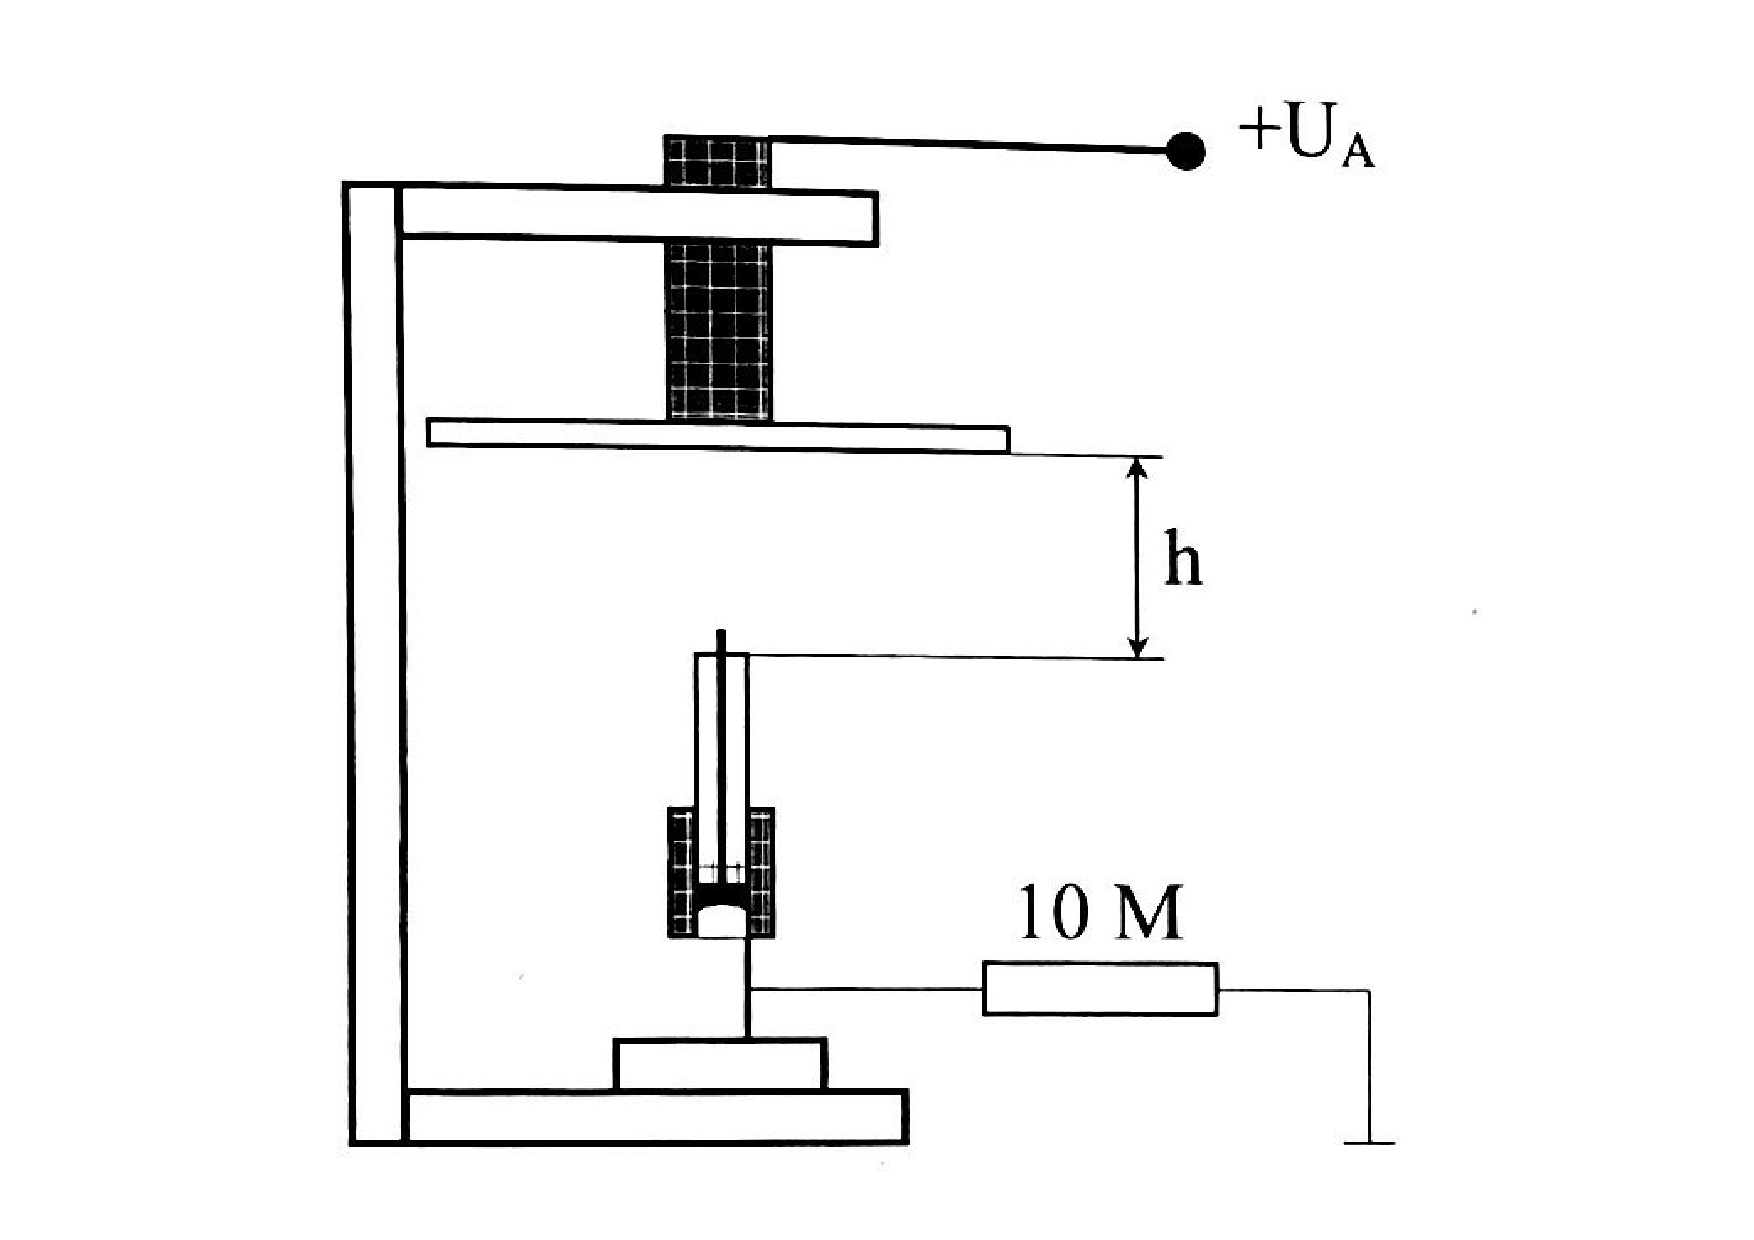
\includegraphics[width=1\linewidth]{p4.pdf}
				\caption{Схема установки для проведения травления}
				\label{default}
			\end{minipage}
			\begin{minipage}[h]{0.4\linewidth}
				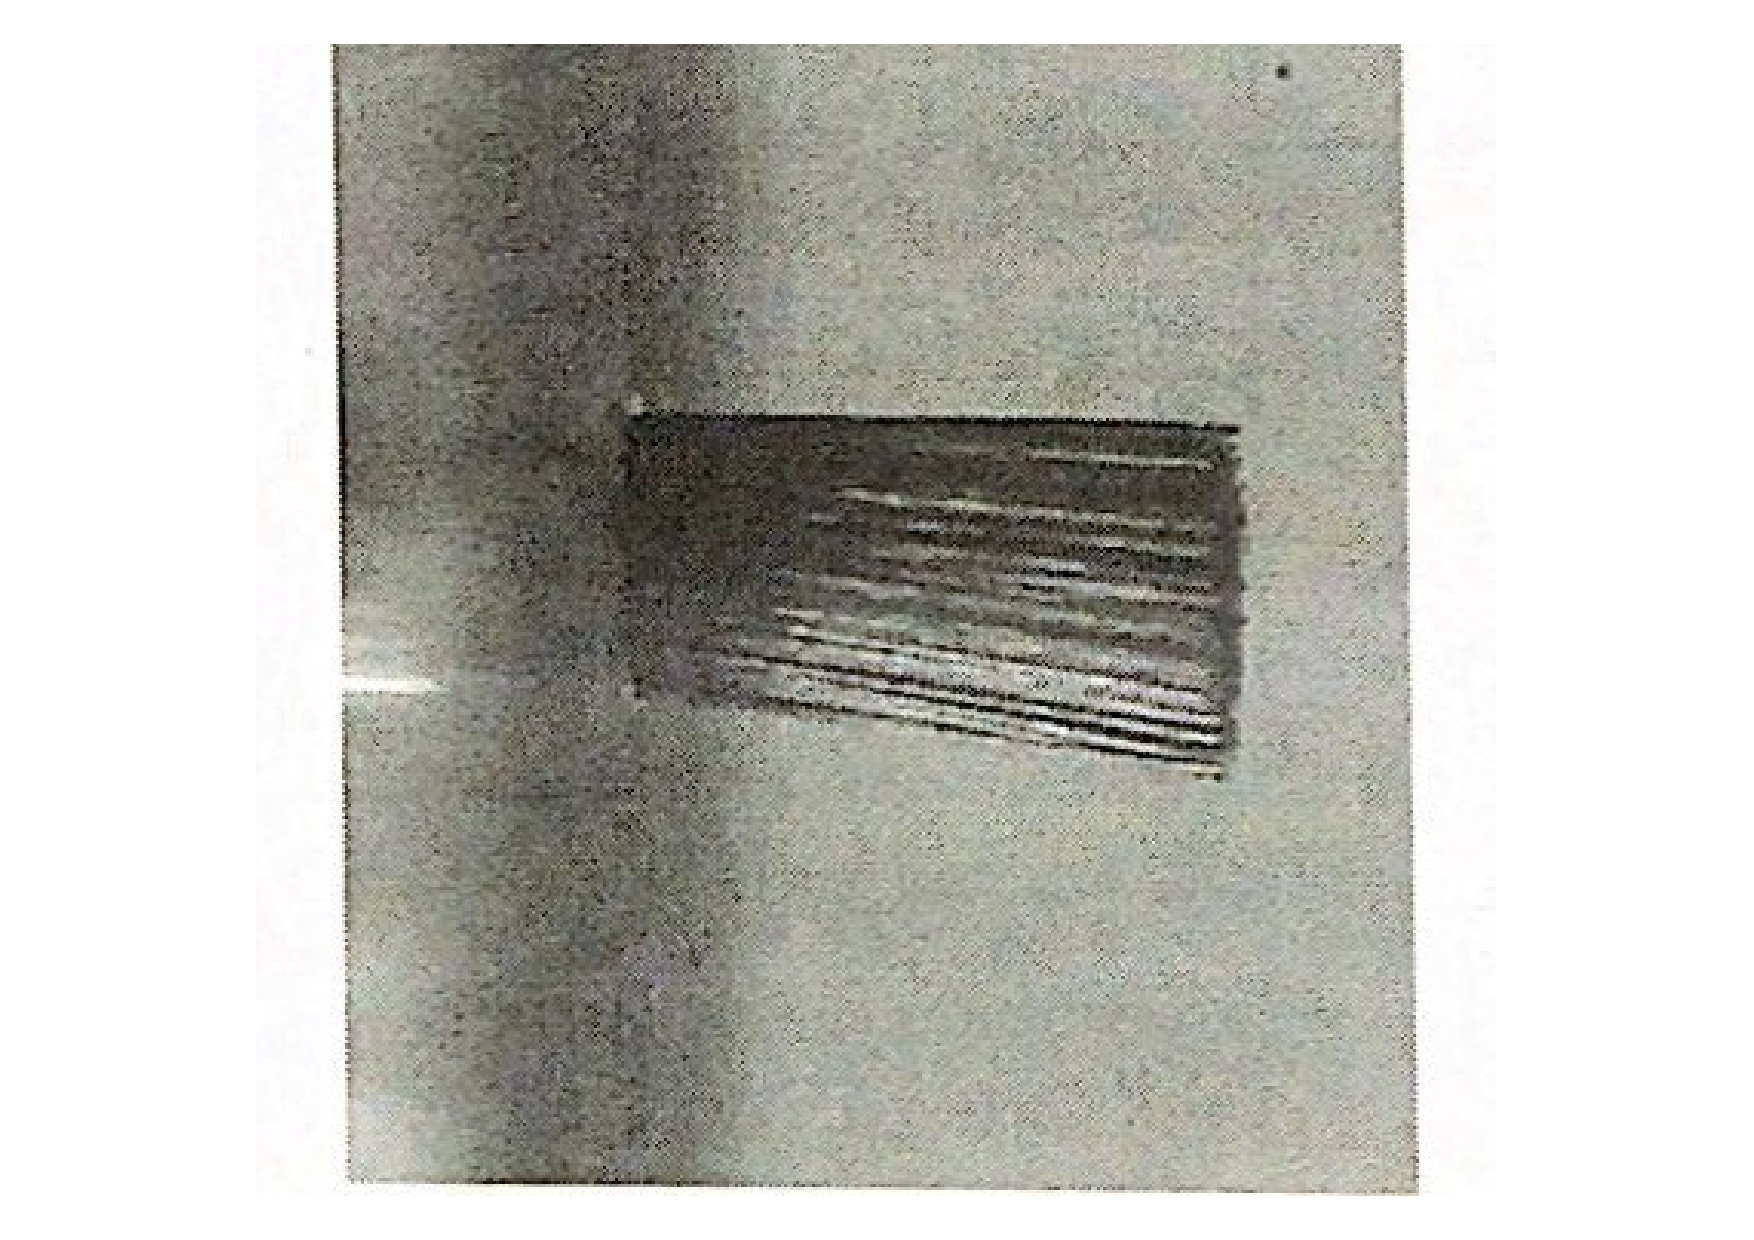
\includegraphics[width=1\linewidth]{do.pdf}
				\caption{До травления} 
				\label{do}
			\end{minipage}
			\hfill 
			\begin{minipage}[h]{0.25\linewidth}
				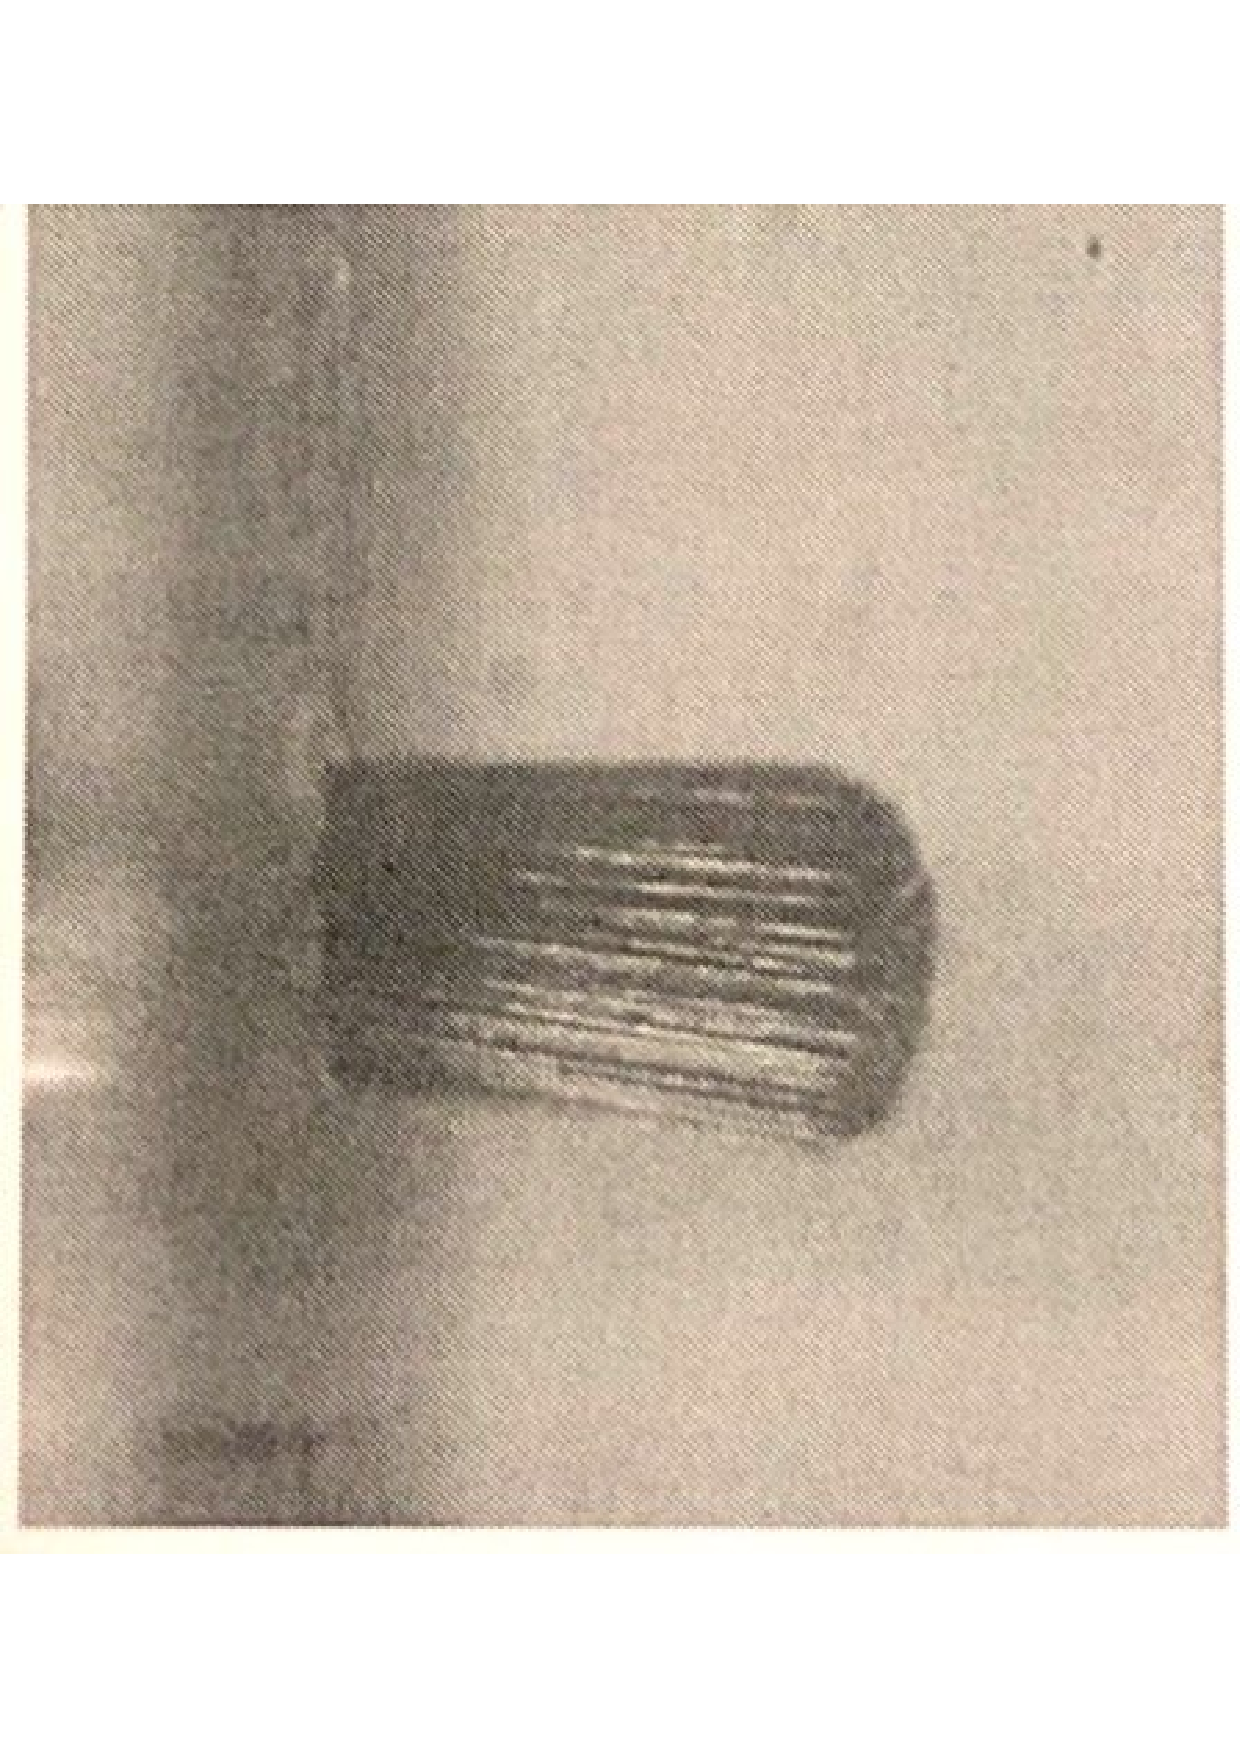
\includegraphics[width=1\linewidth]{posle.pdf}
				\caption{После травления}
				\label{posle}
			\end{minipage}
			\end{center}
		\end{figure}

	\end{itemize}
	

	\item \textbf{Привести способ расчета площади катода.}
	
	Можно найти коэффициент наклона прямой в координатах Фаулера-Нордгейма и по формуле 
	$$tg\alpha = -0.683 \cdot \frac{\phi^{3/2}}{\beta}$$
	при известной работе выхода $\phi$ можем найти формфактор 
	$$\beta = \frac{1}{k \cdot r \cdot \ln{\frac{R}{r}}}$$ откуда найдем 
	радиус катода. Далее по формуле $$S = N \cdot \alpha \cdot r^2$$
	найдем площадь $S$.
	
	N - число эмиссионных центров, $\alpha$ - коэффициент, зависящий от формы эмиссионых центров. (Формула для
	$\beta$ выведена в приближении параболического эмиссионного центра, здесь k = 1/2, R - расстояние
	анод-катод).
	\item \textbf{Объяснить физический смысл щелчка в конце измерения ВАХ.}

	\item \textbf{Привести зависимость автоэмиссионного тока от времени и дать пояснения участкам}.
	
	\item \textbf{Есть эмиссионная лампа с модулятором. Напряжение на аноде фиксировано ($U_A$ = 10 кВ, 
	но это не особо важно), а на катоде повышается. На модуляторе присутствует небольшой потенциал. 
	В результате всего этого со временем на катоде происходит просадка по току на катоде (на выходе 
	из модулятора). Почему так происходит?}


\end{enumerate}

\end{document}